\chapter*{Wireframes}\addcontentsline{toc}{chapter}{Wireframes}
\label{appendix:wireframes}

\begin{figure}[ht]
    \centering
    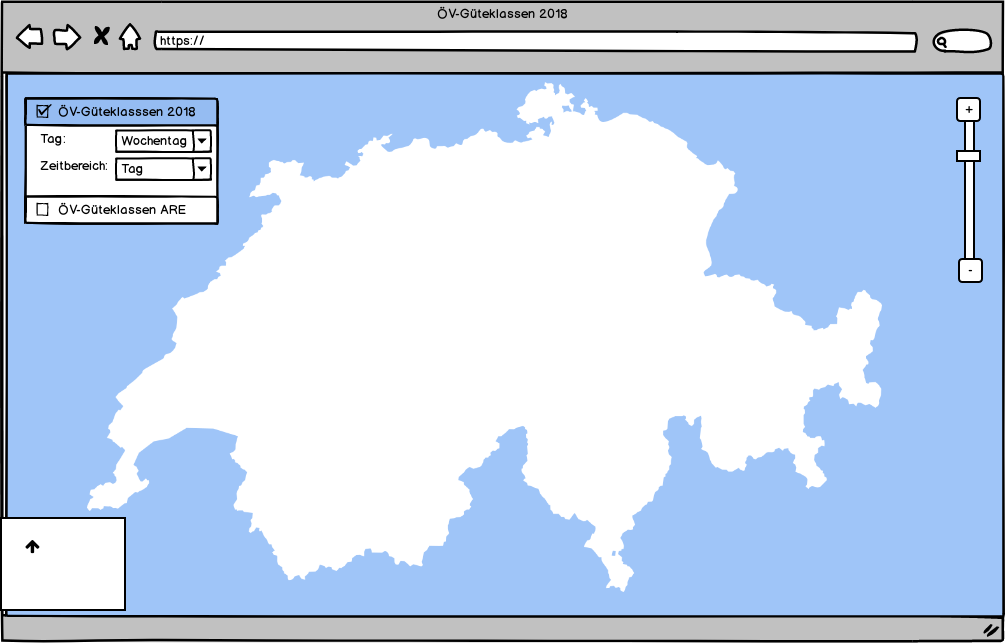
\includegraphics[width=0.8\linewidth]{projectdoc/img/wireframes/standardansicht.png}
    \caption[Wireframe der Standard-Ansicht]{Wireframe der Standard-Ansicht}
    \label{fig:wireframe_main_appendix}
\end{figure}

\begin{figure}[ht]
    \centering
    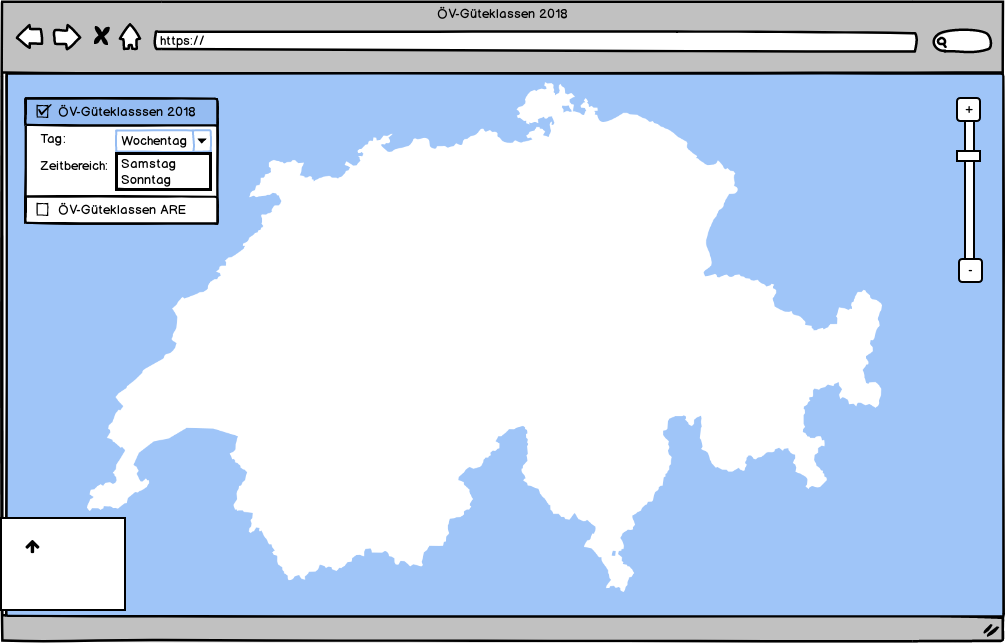
\includegraphics[width=0.8\linewidth]{projectdoc/img/wireframes/tag_auswahl.png}
    \caption[Wireframe zur Auswahl des Tages]{Wireframe zur Auswahl des Tages}
    \label{fig:wireframe_auswahl_tag}
\end{figure}

\begin{figure}[p]
    \centering
    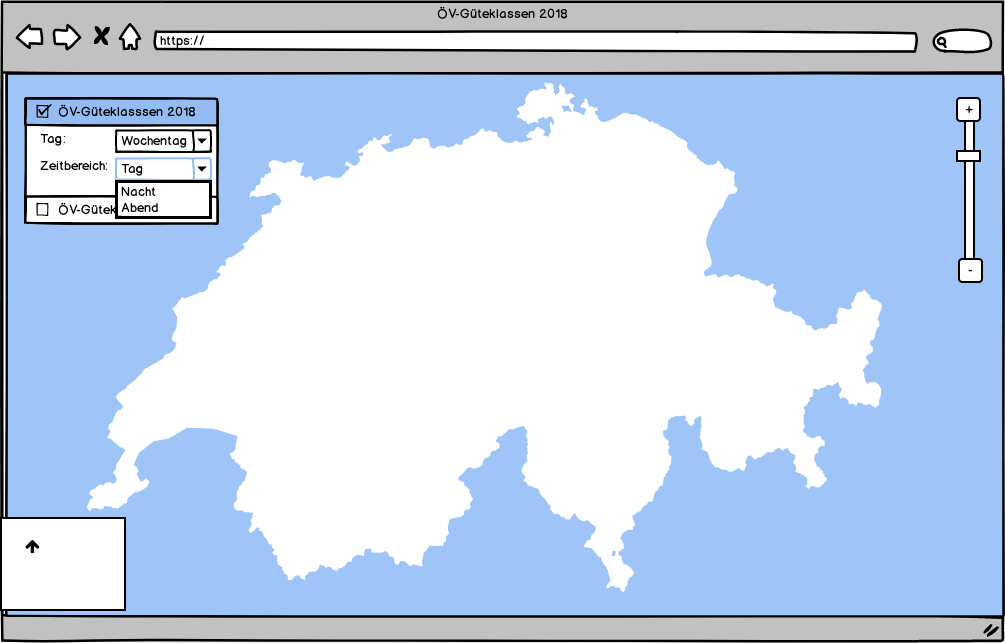
\includegraphics[width=0.8\linewidth]{projectdoc/img/wireframes/zeitbereich_auswahl.png}
    \caption[Wireframe zur Auswahl des Zeitbereichs]{Wireframe zur Auswahl des Zeitbereichs}
    \label{fig:wireframe_auswahl_zeitbereich}
\end{figure}

\begin{figure}[p]
    \centering
    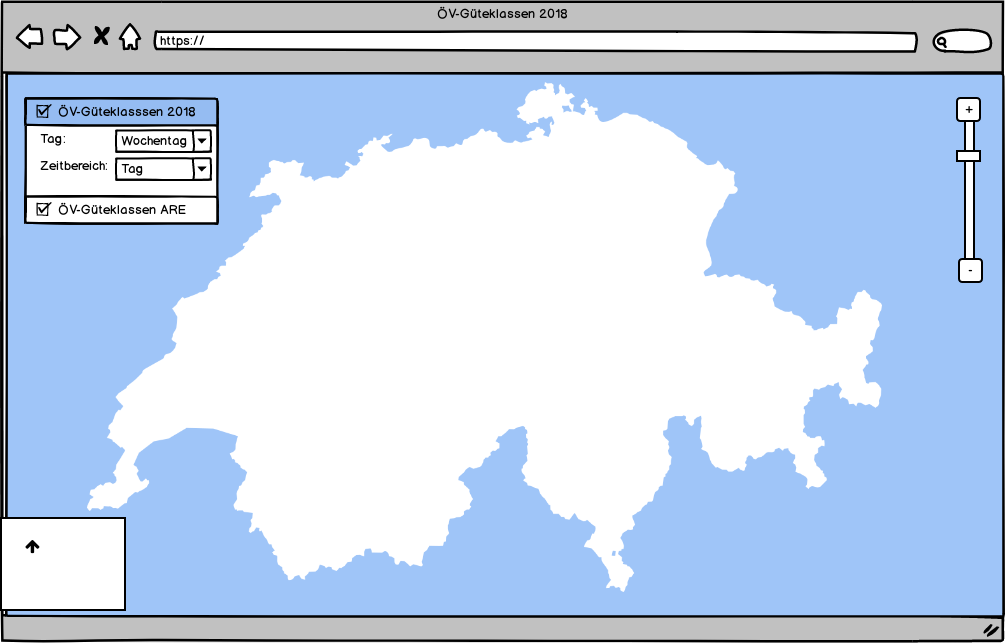
\includegraphics[width=0.8\linewidth]{projectdoc/img/wireframes/are_selected.png}
    \caption[Wireframe, wenn ÖV-Güteklassen ARE ausgewählt wird]{Wireframe, wenn ÖV-Güteklassen ARE ausgewählt wird}
    \label{fig:wireframe_are_selected}
\end{figure}

\begin{figure}[p]
    \centering
    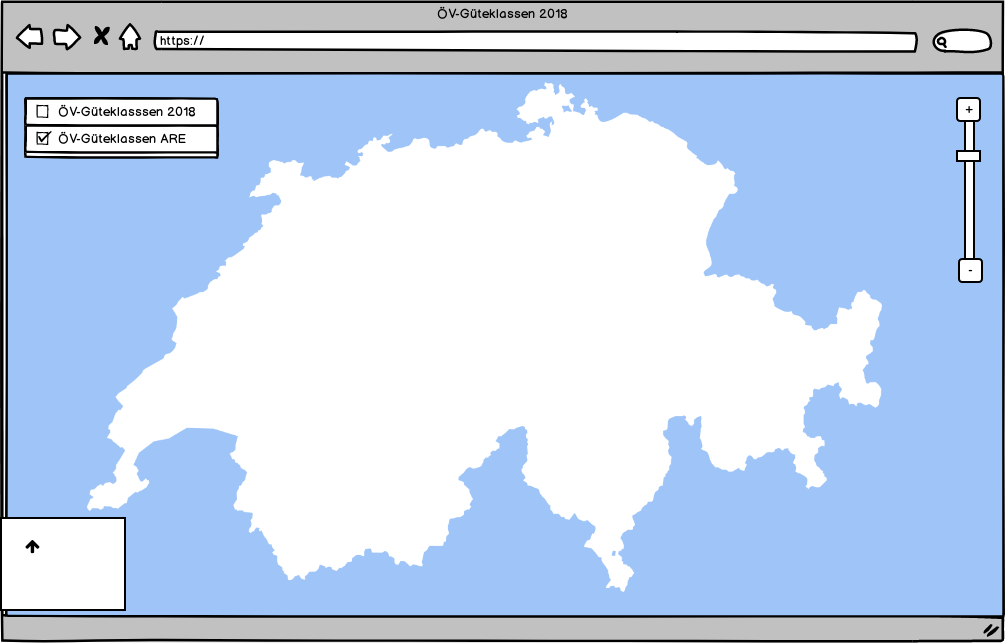
\includegraphics[width=0.8\linewidth]{projectdoc/img/wireframes/only_ARE.png}
    \caption[Wireframe, wenn nur die ÖV-Güteklassen ARE angewählt sind]{Wireframe, wenn nur die ÖV-Güteklassen ARE angewählt sind}
    \label{fig:wireframe_delesected}
\end{figure}

\begin{figure}[p]
    \centering
    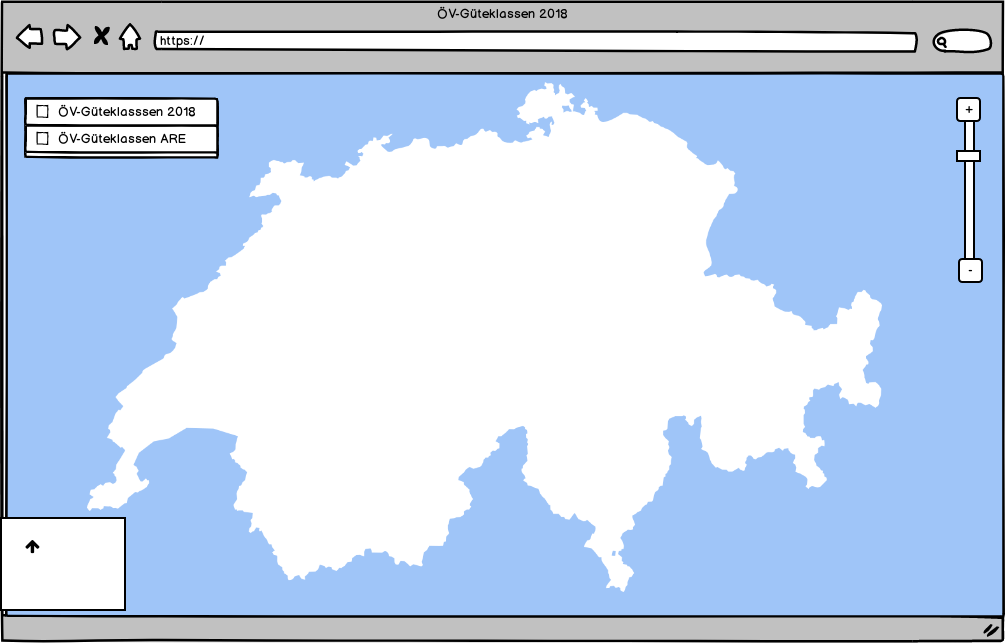
\includegraphics[width=0.8\linewidth]{projectdoc/img/wireframes/deselected.png}
    \caption[Wireframe, wenn alle Ansichten ausgeblendet werden]{Wireframe, wenn alle Ansichten ausgeblendet werden}
    \label{fig:wireframe_delesected}
\end{figure}